\documentclass[tikz,dvipsnames]{standalone}
\usetikzlibrary{backgrounds}
\usetikzlibrary{calc,positioning}

\begin{document}
 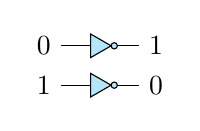
\begin{tikzpicture}[
    show background rectangle,
    tight background=0,
    background rectangle/.style={fill=white},
 ]
    \node (X0)  {$0$};
    \node[right=of X0]  (Y0) {$1$};
    \draw (X0) -- (Y0);
    \filldraw[fill=cyan!30] ($(X0)!0.6!(Y0)$)-- 
        ++(150:0.3) -- ++(270:0.3)
        -- cycle 
        ++(0.04,0) 
        circle (0.04) ;
    
    \node at (0,-0.5) (X1) {$1$};
    \node[right=of X1] (Y1) {$0$};
    \draw (X1) -- (Y1);    
    \filldraw[fill=cyan!30] ($(X1)!0.6!(Y1)$)--  
        ++(150:0.3) -- ++(270:0.3) -- cycle 
        ++(0.04,0) circle (0.04) ;

   
   
\end{tikzpicture}
\end{document}
